\documentclass[11pt,a4paper]{article}

\usepackage[utf8]{inputenc}
\usepackage[ngerman]{babel}
\usepackage{amsmath}
\usepackage{amsthm}
\usepackage{graphicx}
\usepackage[export]{adjustbox}
\graphicspath{ {./images/} }

\title{ARJA: Automated Repair of Java Programs via
Multi-Objective Genetic Programming \\[0.5em] \large{Seminar zu "Machine Learning in Software Eningeering'' \\[0.5em]} }

\author{Paul Groß, David Riemer, Felix Groß}

\date{Sommersemester 2023}

\begin{document}
\maketitle

\section{Einführung in die Funktionsweise von ARJA}
Um die Funktionsweise von ARJA tiefgründig und umfassend zu verstehen, ist es wichtig, die Grundkonzepte und Grundbegriffe in den komplexen Bereichen des Machine Learnings sowie genetischen Algorithmen zu verstehen. Beide Teilgebiete sind wichtige Konzepte in dem Arbeitsfeld der künstlichen Intelligenz und werden dafür eingesetzt, komplexe Probleme zu lösen und Muster in Daten zu erkennen. 
\subsection{Einführung in Machine Learning und genetische Algorithmen}
Sowohl ML, als auch GA umfassen Systemkomponenten, die operatives Datenmaterial zur Informations- und letztlich Wissensgenerierung aufbereiten und speichern sowie Auswertungsund Präsentationsfunktionalität anbieten. Anders gesagt: Machine Learning umfasst den nichttrivialen Prozess der Identifikation gültiger, neuer potentiell nützlicher und letztlich verständlicher Muster in Datenbeständen\footnote{Fayyad et al, The KDD Process für Extracting Useful Knowledge from Volumes of Data; in: Communications of the ACM, Vol. 39, November 1996
}“. Typische Verfahren im Machine Learning, bzw. Data Mining bilden die Clusteranalyse, Entscheidungsbaumverfahren, Assoziationsanalyse, Neuronale Netze oder auch die Regressionsanalyse, wobei in dieser Ausarbeitung für das bessere Verständnis von ARJA besonders auf das Entscheidungsbaumverfahren eingegangen werden soll. Zunächst sollen einige Grundbegriffe erläutert werden. \\ 

\subsubsection{Machine Learning}
Maschinelles Lernen lässt sich in verschiedene Arten unterteilen:
Supervised learning beschreibt ein Konzept des maschinellen Lernens, bei dem ein Modell anhand eines vorgegeben Datensatzes eine Zielfunktion $f$ bildet, die dann ein Objekt O mit einer Menge an Attributen $x$ zu einer vordefinierten Klasse zuordnen kann\footnote{Tan; Steinbach; Kumar: Introduction to Data Mining, Addison-Wesley, 2005}.
\begin{figure}[h]
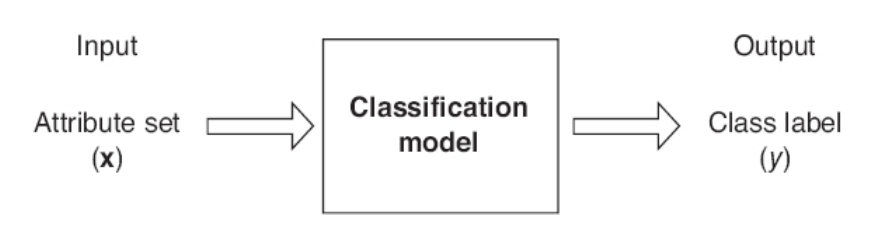
\includegraphics[width=100mm,scale=1, center]{entscheidungsbaum_diagramm.png}
\caption{Visalisierung eines klassischen Klassifikationsmodells}
\label{fig:figure1}
\end{figure}
\\\\Ein durchaus beliebtes Verfahren dieser Methode bilden sogenannte Entscheidungsbäume. 
Diese stellen eine Baumstruktur dar, in der jeder Knoten eine Bedingung repräsentiert und jeder Ast einen möglichen Ausgang oder eine weitere Entscheidung darstellt. Am Ende der Äste werden die Vorhersagen oder Entscheidungen getroffen.
Ein Entscheidungsbaum besteht aus folgenden Elementen:
\begin{itemize}

\item Wurzelknoten: Der oberste Knoten des Baums, von dem aus der Baum beginnt. Er stellt die erste Bedingung dar, anhand derer eine Entscheidung getroffen wird.
\item Innere Knoten: Die nachfolgenden Knoten im Baum, die weitere Bedingungen repräsentieren. Sie teilen den Datenfluss basierend auf bestimmten Merkmalen auf.
\item Blattknoten: Die Endknoten des Baums, die die Vorhersagen oder Entscheidungen repräsentieren. Sie enthalten die Ausgabe oder Klasse, die dem gegebenen Datenpunkt zugeordnet wird.
\end{itemize}
\begin{figure}[h!]
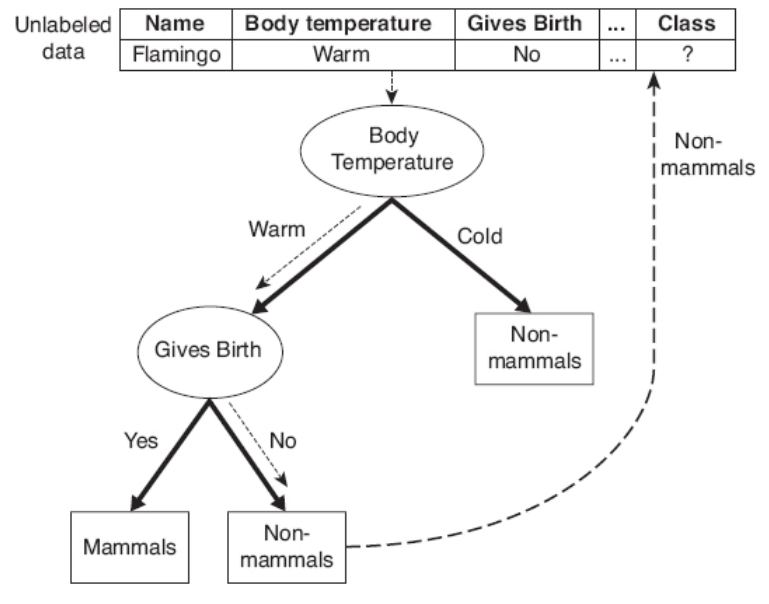
\includegraphics[width=70mm, scale=0.3, center]{entscheidungsbaum.png}
\caption{Ein Entscheidungsbaum zur Klassifikation ob ein Lebewesen ein Säugetier ist, oder nicht}
\label{fig:figure2}
\end{figure}
Die Konstruktion eines Entscheidungsbaums erfolgt in der Regel durch rekursive Teilung des Datensatzes basierend auf bestimmten Merkmalen. Der Algorithmus wählt die besten Bedingungen aus, um die Daten in den einzelnen Schritten aufzuteilen, wobei das Ziel darin besteht, die homogensten Teilmengen an Daten zu erhalten.
\subsubsection{Das Problem des Overfitting}
Ein wichtiger Aspekt bei der Verwendung von Entscheidungsbäumen ist die Vermeidung von Überanpassung (Overfitting). Überanpassung tritt auf, wenn der Baum zu stark auf die Trainingsdaten angepasst ist und nicht in der Lage ist, auf die neuen Daten gut zu generalisieren.  \\Techniken wie Pruning, Regularisierung oder Ensemble-Methoden wie Random Forests können verwendet werden, um Überanpassung zu reduzieren und die Leistung des Entscheidungsbaums zu verbessern.
\begin{figure}[h!]
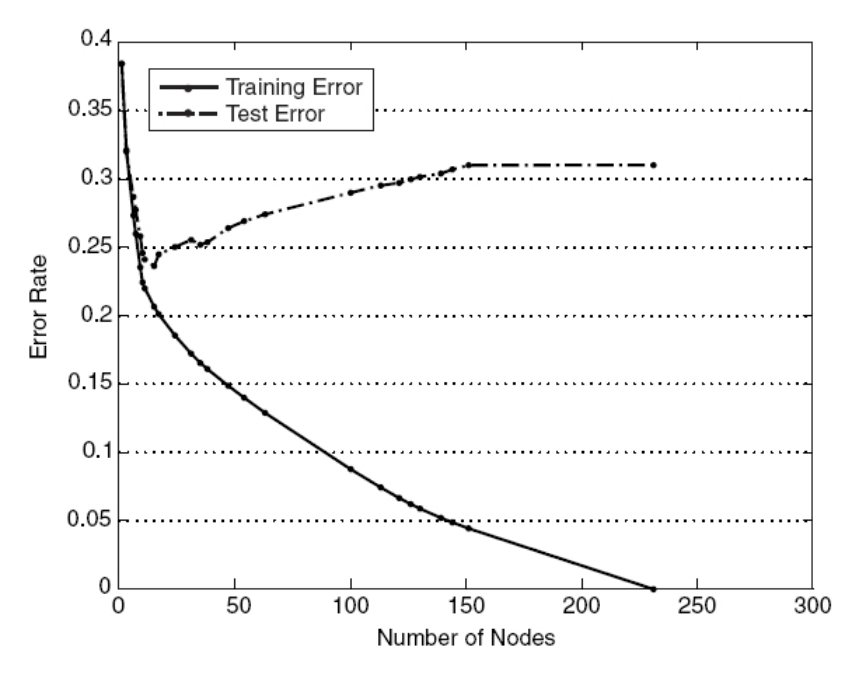
\includegraphics[width=70mm,scale=0.3, center]{overfitting.png}
\caption{Visualisierung von Overfitting: Es treten weniger Fehler auf den Trainingsdaten auf, jedoch umso mehr auf den Testdaten}
\label{fig:figure3}
\end{figure}
\\Was bei den Entscheidungsbäumen zu einer falschen Klassifikation der Testdaten führen kann, könnte skaliert auf ein Programm wie ARJA fatale Folge für den entworfenen Bugfix haben, da das Programm durch den Patch zwar die Tests besteht, jedoch nicht auf die Anforderungen eines realen Problems eingehen kann. 

\subsubsection{Unsupervised Learning}
Unsupervised learning beschreibt wiederum einen anderen Ansatz. Ziel dieser Lernmethode ist es, verborgene Muster, Strukturen oder Beziehungen in den Daten zu finden und diese zu gruppieren oder zu segmentieren, um wertvolle Einblicke und Erkenntnisse zu gewinnen. 

\section{Nutzung des Softwaresystems}
Dieser Abschnitt befasst sich mit dem Einsatz von ARJA in Software-Entwicklungsprojekten. Es soll gezeigt werden, unter welchen Umständen
es sich lohnt, auf automatische Programmreparatur zurückzugreifen und wie der Workflow für die Entwickler des Projekts aussieht.
\\ \\ \\ \subsection{Einsatzfälle von ARJA in Entwicklungsprojekten Korrektur}
Als Entwickler eines Softwareprojekts ist es in allen Phasen des Softwareentwicklungsprozesses wichtig, eine funktionsfähige Software zu entwickeln oder zu warten.
Test-getriebene Entwicklung ist ein agiler Softwareentwicklungsansatz, bei dem Tests vor der eigentlichen Implementierung des Codes geschrieben werden. Der Ansatz besteht aus einem iterativen und inkrementellen Entwicklungszyklus, der aus den folgenden Schritten besteht:

Zuerst werden die Testfälle anhand der Anforderungen des Programms beschrieben und programmiert; anschließend wird der Code des zu schreibenden Programms so lange geändert, bis das Programm alle gegebenen Tests besteht.

Bei der Entwicklung eines komplexen Programms kann es jedoch vorkommen, dass Tests, welche bei Erstentwicklung noch fehlerfrei abliefen nun Fehler verursachen. Natürlich kann dies auch der Fall sein, wenn der Entwickler oder das Entwicklerteam sich dazu entscheidet, Tests erst nach dem Ausbau der Software zu verfassen. Nun ist es sinnvoll, zu überlegen, in welchen Anwendungsfällen der Einsatz eines automatischen repair-Programms zweckmäßig ist und wann man darauf verzichten sollte.

\subsubsection{Entscheidung anhand äußerlicher Sachverhalte}

Einer der wichtigsten Aspekte in der Softwareentwicklung ist die Zeit. Werden bestimmte Deadlines für Bugfixes, Features, etc. nicht eingehalten kann, dies meist verheerende Folgen im Prozess der Softwareentwicklung haben. Weil man als Entwickler häufig unter Zeitdruck steht, kann die Verwendung automatischer Reparaturwerkzeuge (besonders von ARJA)den Zeitaufwand für das manuelle Beheben von Bugs reduzieren. Dadurch hat der Entwickler mehr Zeit, sich wichtigeren Aufgaben zu widmen.

Ein weiteres Einsatzgebiet für den Einsatz von ARP ist die Ressourcenbeschränkungen: Wenn dem Entwickler das erforderliche Fachwissen oder die Ressourcen fehlen, um bestimmte Fehler manuell zu beheben, können automatische Reparaturwerkzeuge eine nützliche Alternative sein.  Hier sollte man jedoch Vorsicht wallten lassen. Wie man in den kommenden Abschnitten sieht, sind ARPs, inklusive ARJA immer noch fehleranfällig. Der Entwickler sollte sicher gehen, dass der durch das Programm erstellte Patch auch wirklich den Bug im System gefixed hat und kein Fehler, z. B. in Form von overfitting entstanden ist.

\subsubsection{Entscheidung anhand des Codes}

Abgesehen von Kriterien der äußerlichen Natur ist es natürlich umso wichtiger Code-spezifische Sachverhalte zu nennen:

Wenn zum Beispiel ein Test gehäuft fehlschlägt, ist es gut möglich, dass ein ARP besser in der Lage ist, das Fehlermuster zu erkennen und zu korrigieren. Dies liegt in der Natur des Machine Learnings.

Außerdem sollte man bei großen Codebasen abwägen, ob die manuelle Fehlersuche optimaler ist als, die Verwendung von ARPs und eine anschließende Analyse des entstandenen Patches. Fehlende Code-Kommentare, redundanter Code, Nichteinhalten der ISO-Normen und viele weitere Faktoren können Gründe dafür sein, wieso das Programm für einen Entwickler nur schwierig lesbar ist. Da ARJA das Programm aber nicht wie ein Mensch übergeht, sondern als einen „abstract syntax tree“ repräsentiert, kann es hier durchaus effizienter sein, ein ARP anzuwenden, gerade bei immer komplexer werdenden Softwaresystemen. Daran anschließen kann man die Legacy-Code-Wartung:
Bei der Wartung von Legacy-Code, der oft wenig oder keine Dokumentation aufweist, können automatische Reparaturwerkzeuge helfen, Fehler zu finden und zu beheben. Sie können auch bei der Verbesserung der Codequalität und Strukturierung älterer Codebasen unterstützen.

Letzten Endes liegt es in der Hand des Entwicklers oder des Entwicklerteams zu entscheiden, ob ein ARP eingesetzt werden sollte oder nicht. Das auf den ersten Blick durchaus effizientere Bugfixing sollte unter keinen Umständen unkontrolliert bleiben und kann unter Umständen mehr Arbeit nach sich ziehen, als ein manuelles Fixen des Codes, wie das folgende Kapitel verdeutlichen soll.
\subsection{Bedienung des Systems als Entwickler und Ausblick}
Figur x beschreibt ein typisches Ablaufszenario für den Einsatz von ARJA als Entwickler.
\begin{figure}[h!]
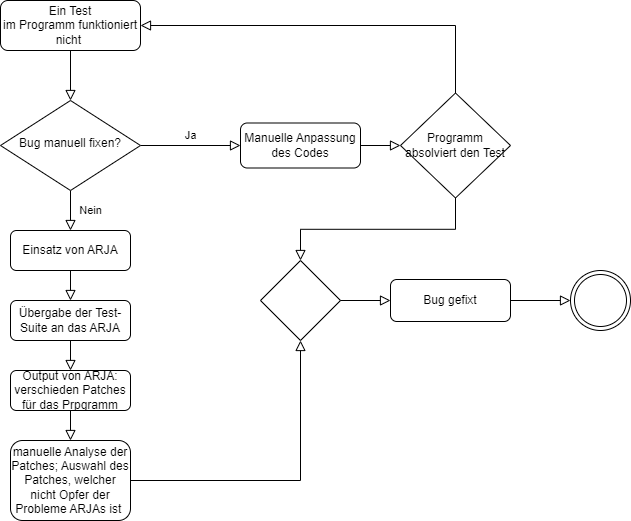
\includegraphics[width=100mm,scale=0.3, center]{ablauf.png}
\caption{Ein typisches Ablaufszenario für den Einsatz von ARJA als Entwickler}
\label{fig:figure4}
\end{figure}

Es fällt auf, dass der Einsatz eines automatisierten Programms für die Fehlerbehebung auf den ersten Blick zwar als die deutlich sparsamere Variante erscheint, aber in manchen Einzelfällen einige Schritte mit sich bringt, welche eventuell komplexer und aufwändiger sind, als die manuelle Behebung des Problems. 

\subsubsection{Ausblick}
Unterstützende Programme beim Programmieren können weit mehr als nur das Beheben von Fehlern und Bugs leisten. Sie bieten eine Vielzahl von Funktionen und Werkzeugen, um den Entwicklungsprozess effizienter und produktiver zu gestalten.
Optimal wäre es für den Workflow eine Balance aus der eigenen Entwicklung und der Nutzung des passenden Programms für die gegebene Problemstellung zu finden und deren Vorteile gezielt zu nutzen. Dies kann man anhand eines kontrollierten Experiments von GitHub erkennen. In diesem wurden 95 Entwickler zufällig in zwei Gruppen eingeteilt und gemessen, wie lange die beiden Gruppen durchschnittlich für ein gegebenes Problem brauchten.
Eine Hälfte hatte Zugriff auf den GitHubCopilot, die andere nicht. Die Ergebnisse zeigen eine signifikante Steigerung der Produktivität, bei der Nutzung eines AI-gesteuerten Entwicklungs-Tools. \footnote{https://github.blog/2022-09-07-research-quantifying-github-copilots-impact-on-developer-productivity-and-happiness/}
\begin{figure}[h!]
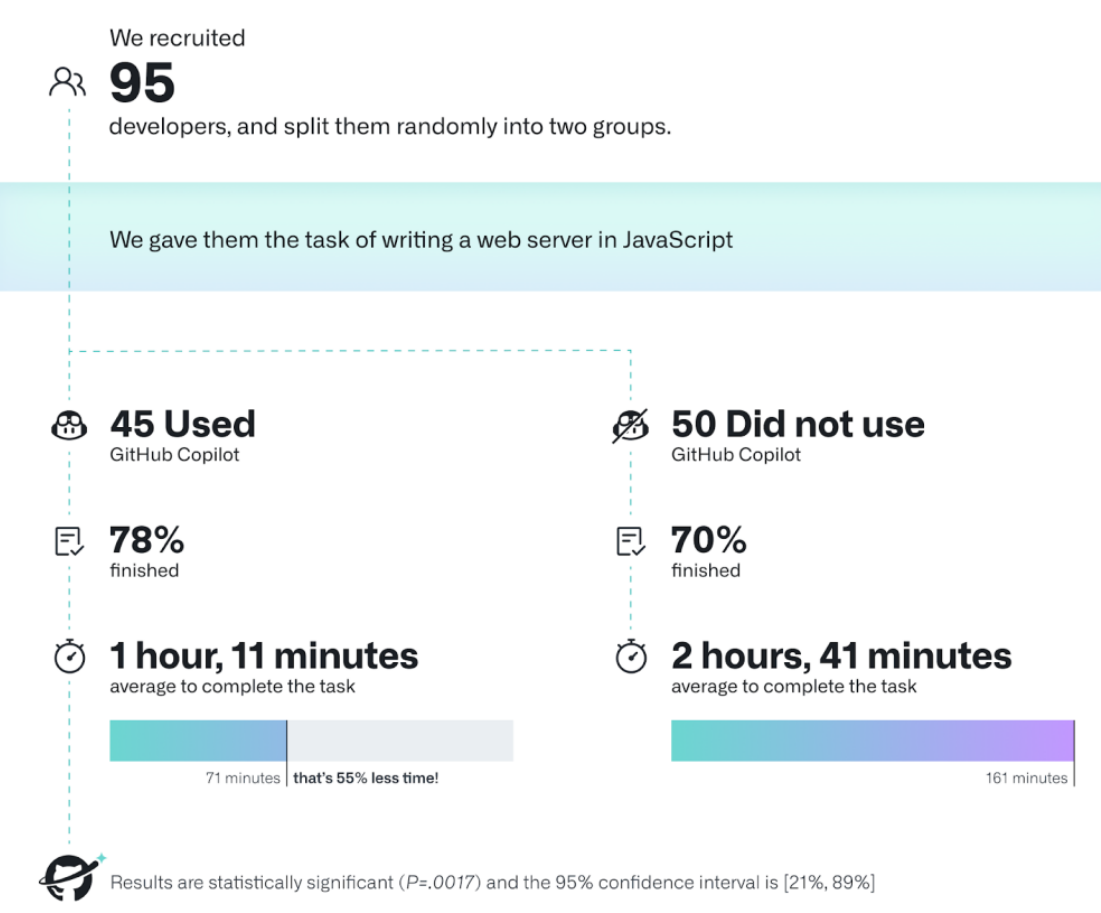
\includegraphics[width=100mm,scale=0.3, center]{copilot.png}
\caption{Ergebnisse des Experiments von GitHub}
\label{fig:figure5}
\end{figure}






\bibliographystyle{abbrv}
\bibliography{seminar}

\end{document}
